%************************************************
\chapter{Representación de variable discreta}\label{ch:DVR}
% ************************************************
Existen diferentes métodos numéricos para resolver la ecuación de Schrödinger dependiente del tiempo \autoref{eq:TDSE ket}. En esta capítulo se desarrollará un método particular conocido como el método de \textbf{representación de variable discreta}, \acs{DVR} \cite{Light1985,Light1992} por sus siglas en inglés.
\\\\
Formalmente, el espacio de Hilbert de las funciones de onda es infinito, sin embargo, para resolver y tratar problemas numéricamente, es necesario hacer un truncamiento de la dimensión del espacio a un número finito $N$. Este espacio tiene el mismo formalismo de la mecánica cuántica, pues la dimensión del espacio de Hilbert está dado por las distintas alternativas que puede tomar el sistema físico en cuestión, de manera que este espacio de dimensión $N$ puede ser un espacio completo para otro problema en mecánica cuántica. Por ejemplo, si $N=2$, el espacio generado puede verse como el espacio de Hilbert asociado al problema de la medición del espín en los átomos de plata \cite{Gerlach1922}.

\section{Proyección espectral y colocación}
Una función de onda y sus operadores se pueden representar mediante una base de funciones ortogonales, a esta base se le conoce como \textbf{base espectral}:
$$\{\phi_i(x)\}_{i=1}^{N},$$
que, por ser funciones ortogonales cumplen que:
$$\bra{\phi_i(x)}\ket{\phi_j(x)} = \delta_{ij}.$$
Como se mencionó anteriormente, la dimensión del espacio de Hilbert se debe reducir a un número finito $N$, esta reducción de dimensión se puede expresar mediante un \textbf{operador de proyección}:

\begin{equation}
  \label{eq:operadorproyeccion}
  P_N = \sum_{n=1}^N\ket{\phi_n}\bra{\phi_n}.
\end{equation}

Mediante el operador $P_N$ se puede mapear la dinámica del espacio de Hilbert al espacio reducido de Hilbert, en particular, es de interés para resolver la \autoref{eq:TDSE ket} conocer cómo se representa el operador Hamiltoniano en su representación matricial:
\begin{equation}
  \label{eq:Hamiltoniano}
  H = \frac{\hat{p}^2}{2m}+V(\hat{x}).
\end{equation}

Asumiendo que la matriz de elementos $\bra{\phi_m}H\ket{\phi_n}$ es conocida dada la base espectral, el Hamiltoniano en el espacio reducido de Hilbert se puede representar como:

\begin{equation}
  \label{eq:Hamiltonianored}
  H_N = P_NHP_N.
\end{equation}

La ecuación de Schrödinger dependiente del tiempo:

\begin{equation}
  \label{eq:tdse-1}
  i\hbar\frac{\partial \psi}{\partial t} = H \psi,
\end{equation}

\noindent puede escribirse como un conjunto de dos ecuaciones diferenciales acopladas a partir de las siguientes definiciones \cite{Tannor:2006}:

\begin{equation}
  \label{eq:acop1}
  Q_N = \mathbb{1} - P_N,
\end{equation}

\begin{equation}
  \label{eq:acop2}
  \psi_N = P_N\psi,
\end{equation}

\begin{equation}
  \label{eq:acop3}
  \psi_{\perp}=Q_N\psi = \psi - \psi_{N},
\end{equation}

\noindent de la \autoref{eq:acop3} se sigue que: $\psi = \psi_N + \psi_{\perp}$, sustituyendo en la \autoref{eq:tdse-1} se tiene:
\begin{equation}
  \label{eq:tdse-2}
  i\hbar\frac{\partial (\psi_N + \psi_{\perp})}{\partial t} = H (\psi_N + \psi_{\perp}),
\end{equation}

\noindent multiplicando por el operador $P_N$ por la izquierda en ambos lados se obtiene:
\begin{equation}
   \label{eq:tdse-3}
  i\hbar\frac{\partial (P_N \psi_N + P_N \psi_{\perp})}{\partial t} = P_NH (\psi_N + \psi_{\perp}),
\end{equation}

\noindent por definición $P_N \psi_{\perp}= P_NQ_N\psi = P_N(\mathbb{1}-P_N)\psi = (P_N - P_N^2)\psi = (P_N-P_N)\psi=0$, pues $P_N$ es un operador de proyección, también se sigue que $P_N\psi_N = P_N P_N \psi = P_N^2 \psi = P_N\psi = \psi_N$
De esta manera la \autoref{eq:tdse-3} se convierte en:

\begin{equation}
   \label{eq:tdse-4}
  i\hbar\frac{\partial \psi_N}{\partial t} = P_NH (\psi_N + \psi_{\perp}),
\end{equation}

multiplicando por $\mathbb{1}=P_N + Q_N$ en el lado derecho de la ecuación se sigue:
\begin{align}
  \label{eq:tdse-5}
 i\hbar\frac{\partial \psi_N}{\partial t}&= P_NH(P_N + Q_N) (\psi_N + \psi_{\perp}), \nonumber  \\ 
                                         &= (P_NHP_N + P_NHQ_N)(\psi_N + \psi_{\perp}), \nonumber \\
  &= P_NHP_N\psi_N + P_NHQ_N\psi_N + P_NHQ_N\psi_{\perp} + P_NHQ_N\psi_{\perp}.
\end{align}

\noindent como se mostró anteriormente $P_N\psi_{\perp}=0$, además $Q_N \psi_N = (\mathbb{1}-P_N)\psi_N = \psi_N - P_N\psi_N = \psi_N - \psi_N = 0$, de esta manera el segundo y tercer término del lado derecho en la \autoref{eq:tdse-5} se cancelan y se sigue que:

\begin{equation}
  \label{eq:tdse-p1}
  i\hbar\frac{\partial \psi_N}{\partial t} = P_NHP_N\psi_N  + P_NHQ_N\psi_{\perp}.
\end{equation}

Por otro lado, multiplicando el operador $Q_N$ por la izquierda en ambos lados de la \autoref{eq:tdse-2} se tiene:

\begin{align}
   \label{eq:tdse-6}
  i\hbar\frac{\partial (Q_N \psi_N + Q_N \psi_{\perp})}{\partial t} &= Q_NH (\psi_N + \psi_{\perp}), \nonumber \\
  i\hbar\frac{\partial \psi_{\perp}}{\partial t} &= Q_NH (\psi_N + \psi_{\perp}),
\end{align}

\noindent multiplicando por $\mathbb{1}=P_N + Q_N$ en el lado derecho de la ecuación se sigue:
\begin{align}
  \label{eq:tdse-7}
  i\hbar\frac{\partial \psi_{\perp}}{\partial t}&= Q_NH(P_N + Q_N) (\psi_N + \psi_{\perp}), \nonumber  \\ 
                                         &= (Q_NHP_N + Q_NHQ_N)(\psi_N + \psi_{\perp}), \nonumber \\
                                          &= Q_NHP_N\psi_N + Q_NHQ_N\psi_N + Q_NHP_N\psi_{\perp} + Q_NHQ_N\psi_{\perp}.
\end{align}

\noindent por los argumentos anteriores, el segundo y tercer término del lado derecho de la \autoref{eq:tdse-7} se cancelan, obteniendo:

\begin{equation}
  \label{eq:tdse-p2}
  i\hbar\frac{\partial \psi_{\perp}}{\partial t} = Q_NHP_N\psi_N + Q_NHQ_N\psi_{\perp},
\end{equation}

de esta manera la \autoref{eq:tdse-p1} y la \autoref{eq:tdse-p2} son un conjunto de dos ecuaciones diferenciales acopladas.
\\
Para este trabajo se usará la aproximación de Galerkin \cite{Gottlieb}, en donde se desprecia la contribución de $\psi_{\perp}$, de esta forma, la \acs{TDSE} a resolver es:
\begin{tcolorbox}[colback=CTtitle!5!white,colframe=CTtitle!85!white]%,title=\centering{Ecuación de Schrödinger Dependiente del Tiempo para un estado}]
\begin{equation}
\label{eq:TDSEN}
i\hbar \frac{\partial \psi_N}{\partial t} = P_NHP_N\psi_N
\end{equation}
\end{tcolorbox}

\subsection{Representación de la función de onda bajo el operador de proyección}

Una función de onda $\psi(x)$ se puede escribir como una suma infinita en términos de funciones ortonormales $\phi_i$:
\begin{equation}
  \label{eq:wavefuninf}
  \psi(x) = \sum_{n=1}^{\infty}a_n\phi_n(x),
\end{equation}
con:
\[ \int \phi_m^*(x)\phi_n(x)dx = \delta_{mn}, \]
\[ a_n = \int \phi_n^*(x)\psi(x)dx,\]
para $m,n=1,2,3,\dots, \infty$.
\\
\\
Utilizando la definición del operador de proyección de la \autoref{eq:operadorproyeccion}, se puede probar que:
\begin{equation}
  \label{eq:wavepacketinit}
  \psi_N(x) = P_N\psi(x)=\sum_{n=1}^{N}a_n\phi_n(x).
\end{equation}

\subsection{Definición del proyector de colocación}\label{sec:collocation}
Dado un conjunto de puntos en el espacio de posiciones $\{x_i\}$ con $i=1,2,3,\dots, N$, la siguiente relación:
\begin{equation}
  \label{eq:wavefunexp}
  \psi_N(x_i) = P_N\psi(x_i)=\sum_{n=1}^{N}b_n\phi_n(x_i) = \psi(x_i),
\end{equation}

\noindent está asociada a la \textbf{colocación}\footnote{Los \textbf{métodos de colocación} son soluciones numéricas de un conjunto de ecuaciones, cuya solución resulta ser exacta en un conjunto discreto de puntos llamados puntos de colocación.\cite{Tannor:2006}} del operador de proyección, y los puntos $\{x_i\}$ son llamados \textbf{puntos de colocación}. Los coeficientes $b_n$ están determinados por la condición de que: $\psi_N(x)=\psi(x)$ en el conjunto de puntos de colocación.
\\
Es importante notar que los coeficientes $b_n$ son en general distintos a los coeficientes $a_n$ de la \autoref{eq:wavepacketinit}. A pesar de que el operador $P_N$ en la proyección espectral genera el mismo espacio reducido de Hilbert que el operador $P_N$ en la colocación, estos operadores difieren en el estado que producen en el mismo espacio. Si se define:
\begin{equation}
  \label{eq:chi}
  \chi = \psi - \psi_N.
\end{equation}
Para la proyección espectral se tiene que:
\begin{equation}
  \label{eq:ortochi}
  \chi(x) = \sum_{n=1}^{\infty} a_n\phi_n(x) - \sum_{n=1}^{N} a_n\phi_n(x)=\sum_{n=N+1}^{\infty} a_n\phi_n(x),
\end{equation}
de manera que:
\begin{equation}
  \label{eq:puntoorto}
  \bra{\chi}\ket{\psi_N}= \int \left( \sum_{n=N+1}^{\infty} a_n^*\phi_n^*(x)\right) \left( \sum_{m=1}^{N} a_m\phi_m(x) \right)dx = 0,
\end{equation}

\noindent lo que muestra que el proyector espectral es un proyector ortogonal. Por otro lado, si se considera la colocación del proyector:
\begin{equation}
  \label{eq:chinon}
  \chi(x) = \psi - \psi_N = \sum_{n=1}^{\infty} a_n\phi_n(x) - \sum_{n=1}^{N} b_n\phi_n(x),
\end{equation}
el producto está dado por:
\begin{equation}
  \label{eq:puntonon}
  \bra{\chi}\ket{\psi_N}= \int \left(\sum_{n=1}^{\infty} a_n^*\phi_n^*(x) - \sum_{n=1}^{N} b_n^*\phi_n^*(x) \right)
  \left(  \sum_{m=1}^{N} b_m\phi_m(x)  \right) dx \neq 0,
\end{equation}
mostrando así que el proyector de colocación no es un proyector ortogonal. La \autoref{fig:projortoandnon} muestra una interpretación geométrica de lo anterior, en este caso el espacio reducido es $\mathbb{R}^2$, y el vector $(x,y,z) \in \mathbb{R}^3$ es proyectado por dos distintos operadores, uno ortogonal y uno no ortogonal, como se observa, el vector proyectado en ambos casos pertenece al mismo espacio reducido, pero no son el mismo vector \cite{Tannor:2006}.

\begin{figure}[ht]
  \centering
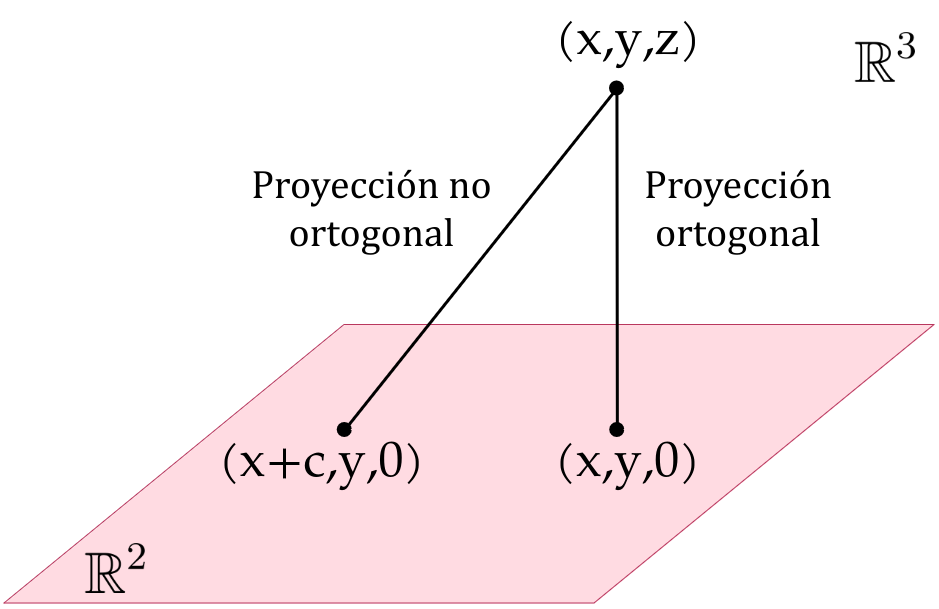
\includegraphics[width=0.6\textwidth]{./img/projortoandnon.drawio.png}
\caption{Interpretación geométrica de una proyección ortogonal y una no ortogonal del un vector en el espacio $\mathbb{R}^3$ al espacio $\mathbb{R}^2$. }
\label{fig:projortoandnon}
\end{figure}

\subsection{Colocación ortogonal}

Un proyector que cumpla con las condiciones de colocación y además sea un proyector ortogonal debe tener funciones $\phi_n(x)$ que satisfagan las relaciones discretas de ortogonalidad definidas en los puntos de colocación \cite{Tannor:2006}:

\begin{equation}
  \label{eq:ortox2}
  \sum_{j=1}^N \phi_m^*(x_j)\phi_n(x_j)\Delta_j = \delta_{mn}, \,\,\, m,n=1,\dots,N,
\end{equation}

\noindent en donde $\Delta_j$ es un factor de peso. Los coeficientes $b_n$ de la \autoref{eq:wavefunexp} pueden encontrarse a partir de la \autoref{eq:ortox2} multiplicando a la izquierda por $\phi_m^*(x_j)\Delta_j$ y sumando sobre $j$:
\begin{equation}
  \label{eq:11.36}
  b_n = \sum_{j=1}^N\psi(x_j)\phi_n^*(x_j)\Delta_j.
\end{equation}
Lo anterior es una buena aproximación discreta a la relación de los coeficientes $a_n$ en la \autoref{eq:wavefuninf}, que cumplen la condición para una proyección ortogonal. Los esquemas que satisfacen la \autoref{eq:ortox2} son llamados \textbf{esquemas de colocación ortogonales}, y pueden ser redefinidos de manera más sencilla de la siguiente manera:
\begin{equation}
  \label{eq:11.37}
  \Phi_n(x_j) \equiv \sqrt{\Delta_j} \phi_n(x_j),
\end{equation}
así, la \autoref{eq:ortox2} puede escribirse como:
\begin{equation}
  \label{eq:11.38}
  \sum_{j=1}^N \Phi_m^*(x_j)\Phi_n(x_j) = \delta_{mn}, \,\,\, m,n=1,\dots,N.
\end{equation}
La ecuación anterior puede escribirse en forma matricial como:
\begin{equation}
  \label{eq:11.39}
  \Phi^{\dag}\Phi=\mathbb{1},
\end{equation}
lo que indica que la transformación $\Phi$ es unitaria, por lo que se tiene también la siguiente relación:
\begin{equation}
  \label{eq:11.40}
  \Phi\Phi^{\dag} = \mathbb{1},
\end{equation}
que puede escribirse de manera extendida como:
\begin{equation}
  \label{eq:11.41}
  \sum_{n=1}^N \Phi_n(x_i)\Phi_n^*(x_j) = \delta_{ij}, \,\,\, i,j=1,\dots,N,
\end{equation}
es importante notar que la ecuación anterior es distinta a la \autoref{eq:11.38}, pues la ecuación \autoref{eq:11.41} implica una relación de ortogonalidad para los diferentes puntos en la malla del espacio de posiciones. La matriz $\Phi$ será llamada matriz de colocación ortogonal.

\section{Base pseudo-espectral}\label{sec:ps-basis}

Una \textbf{base pseudo-espectral}: $\{\theta_j\}_{j=1}^N$ se define como la base de las funciones localizadas espacialmente. La base de funciones ortogonales $\{\phi_n\}_{n=1}^N$, la colocación en la \autoref{eq:wavefunexp}, los puntos de colocación $\{x_i\}_{i=1}^N$, y los factores de peso definidos como $\Delta_j$ con $j=1,\dots,N$, determinan completamente la forma de la base pseudo-espectral. \\
Reemplazando $\Phi_n(x_i)$ por $\phi_n(x)$ en el primer factor de la \autoref{eq:11.41} se definen las funciones pseudo-espectrales base:

\begin{equation}
  \label{eq:11.43}
  \theta_j(x) \equiv \sum_{n=1}^N\phi_n(x)\Phi_n^*(x_j).
\end{equation}

Las funciones $\{\theta_j\}$ son localizadas, cada una alrededor de los diferentes valores $x_j$. De la \autoref{eq:11.43}, \autoref{eq:11.37} y \autoref{eq:11.41} se tiene que las funciones satisfacen:

\begin{equation}
  \label{eq:11.44}
  \theta_j(x_i) = \Delta_j^{-1/2}\delta_{ij}.
\end{equation}

La \autoref{eq:11.43} puede escribirse en notación matricial como:
\begin{equation}
  \label{eq:11.45}
  \Phi^{\dag}\phi(x) = \theta(x),
\end{equation}

\noindent de manera que $\{\theta_j\}$ y $\{\phi_n \}$ son bases que están relacionadas mediante una transformación unitaria $\Phi^{\dag}$ y generan el mismo espacio de Hilbert reducido. Como consecuencia, el operador de proyección es idéntico en ambas bases:
\begin{equation}
  \label{eq:proyecbases}
  P_N = \sum_{n=1}^N\ket{\phi_n}\bra{\phi_n}=\sum_{j=1}^N\ket{\theta_j}\bra{\theta_j}.
\end{equation}

\subsection{Completes y ortogonalidad de las funciones base pseudo-espectrales}
La base de las funciones localizadas $\{\theta_j\}$ cumple las propiedades de ortogonalidad y completes, para mostrar esto se multiplica por $\phi^*_m(x)$ ambos lados de la ecuación \autoref{eq:11.43} y se integra sobre el dominio:
$$ \int \phi^*_m(x) \theta_j(x_j) dx = \int \sum_{n=1}^{N}\phi^*_m(x)\phi_n(x)\Phi^*_n(x_j) dx,$$
\begin{equation}
  \label{eq:11.46}
\bra{\phi_n} \ket{\theta_j} =   \Phi^*_n(x_j). 
\end{equation}
De esta manera, la relación de ortogonalidad es:
\begin{equation}
  \label{eq:11.47}
  \sum_{n=1}^N \Phi_n(x_i)\Phi_n^*(x_j) = \delta_{ij}=\sum_{n=1}^{N}\bra{\theta_i}\ket{\phi_n}\bra{\phi_n}\ket{\theta_j} = \bra{\theta_i}\ket{\theta_j},
\end{equation}
mientras que la de completes está dada por:
\begin{equation}
  \label{eq:11.48}
  \sum_{j=1}^N \Phi_m(x_j)\Phi_n^*(x_j) = \delta_{mn} = \sum_{j=1}^N \bra{\phi_m} \ket{\theta_j} \bra{\theta_j}\ket{\phi_n}.
\end{equation}
La \autoref{eq:11.47} significa que las funciones $\theta_j$ tienen un pico en el valor correspondiente a $x_j$ mientras que se desvanece en cualquier otro punto de la malla $x_i$. La \autoref{eq:11.48} es una relación de completes respecto a la suma sobre todos los puntos de la malla.

\subsection{El proyector de colocación en la base pseudo-espectral}
En la sección \autoref{sec:collocation} se definió el proyector de colocación utilizando la base espectral $\{ \phi_i(x)\}_{i=1}^{N}$, en esta sección se escribirá la relación de colocación en la base pseudo-espectral.
\\

La \autoref{eq:11.43} puede invertirse usando la matriz de transformación unitaria $\Phi$:
\begin{equation}
  \label{eq:11.51}
  \phi_n(x) = \sum_{i=1}^{N}\Phi_n(x_i)\theta_i(x),
\end{equation}
usando esta relación, la \autoref{eq:wavefunexp} y la \autoref{eq:11.37}, se puede reescribir la relación de colocación como:
\begin{equation}
  \label{eq:11.53}
  \psi_N(x) = \sum_{n=1}^N b_n\phi_n(x) = \sum_{i=1}^N \left \{ \sum_{n=1}^Nb_n\Phi_n(x_i)\right\} \theta_i(x),
\end{equation}
\begin{equation}
  \label{eq:11.54}
  \psi_N(x) = \sum_{i=1}^N \psi(x_i)\theta_i(x_i)\Delta_i^{1/2}.
\end{equation}
En los puntos de colocación $\{x_i\}$ se tiene:

\begin{equation}
  \label{eq:11.55}
  \psi_N(x_i) = \sum_{i=1}^N \psi(x_i)\theta_i(x_i)\Delta_i^{1/2},
\end{equation}

\noindent de esta manera se tiene la relación de colocación en la base pseudo-espectral $\{ \theta_i(x)\}_{i=1}^N$.

\section{Algoritmo DVR aplicado a un proceso físico-químico}\label{sec:DVRapp}

En esta sección se aplicarán los conceptos revisados a lo largo del capítulo para resolver un problema físico-químico que involucra potenciales dependientes del tiempo utilizando el método \acs{DVR}. En la \autoref{sec:ProtonTransfer} se describe el modelo físico, en las secciones siguientes se detallan los pasos en el algoritmo \acs{DVR} para resolver la ecuación de Schrödinger dependiente del tiempo correspondiente.
\\
La implementación numérica se realizó en Python 3.9.7 y se encuentra disponible en el repositorio: \href{https://github.com/Jessi-MM/LSTM_PropagatorLearning/blob/main/src/Update_Proton_Transfer_DataGenerate.ipynb}{\faGithub DVR transferencia de protones}

\subsection{Sistema de transferencia de protones}\label{sec:ProtonTransfer}

Los sistemas de \textbf{transferencia de protones} son reacciones presentes en diversos sistemas biológicos y químicos, tales como fotosíntesis natural y artificial \cite{Hoganson1997, AlstrumAcevedo2005}, la oxidación catalítica y producción de hidrógeno molecular \cite{DuBois2011}, y varias reacciones de enzimas \cite{Stubbe2003, Knapp2002}.\\

Estas reacciones involucran la interacción entre una partícula donadora del protón $H^+$ y una partícula aceptora. El Hamiltoniano molecular completo que describe el sistema está dado por:
\begin{align*}
  H &= \sum_i - \frac{\hbar^2 \nabla^2_{e_i}}{2m} + \sum_{j>i} \frac{e^2}{|r_i-r_j|} + \sum_i - \frac{\hbar^2 \nabla^2_{N_i}}{2M_i} + \sum_{j>i} \frac{Z_iZ_je^2}{|R_i-R_j|} - \sum_{ij} \frac{Z_je^2}{|r_i-R_j|}, \\
  & \equiv T_e + V_e + T_N + V_N + V_{eN},
\end{align*}

\noindent en donde las coordenadas $r, \nabla_e$ representan las coordenadas de los electrones y momentos respectivamente, $R,\nabla_N$ representan las coordenadas de los núcleos y sus momentos y $Z_i$ representa la carga nuclear en el núcleo $i$. Los términos en el Hamiltoniano representan la energía cinética de los electrones $T_e$, la energía potencial electrón-electrón $V_e$, la energía cinética de los núcleos $T_N$, la energía potencial núcleo-núcleo $V_n$ y la energía potencial electrón-núcleo $V_{eN}$. \\

Debido a que los núcleos involucrados en el sistema son mucho más pesados que los electrones, su movimiento es muy lento respecto al de los electrones. La aproximación de Born-Oppenheimer \cite{Born1927, LPauling1935} permite tratar al sistema completo como núcleos estacionarios que generan un campo para los electrones, de esta manera, se puede resolver la ecuación de Schrödinger para la parte electrónica y encontrar las superficies de energía potencial o PES, por sus siglas en inglés. Los sistemas de transferencia de protones son, en general, electrónicamente adiabáticos, en el sentido de que ocurren en el estado base, o ground state (GS) en inglés, y no involucran los estados excitados del sistema, o excited states (ES) en inglés \cite{Enzymes}. \\

Una vez obtenido el estado base, se puede resolver la ecuación de Schrödinger para la parte nuclear incluyendo el protón, tomando como potencial resultante el estado base producto de resolver la ecuación de Schrödinger para la parte electrónica y considerando únicamente al protón en el término de energía cinética, debido a que los núcleos han sido considerados estacionarios y su interacción está incluida en el potencial estado base. De manera que el Hamiltoniano puede aproximarse como:

\begin{equation}
  \label{eq:hamApprox}
  H = -\frac{\hbar^2}{2m}\nabla^2_{H^+} + V_{GS}.
\end{equation}

El modelo simplificado en una dimensión de un complejo de enlaces de hidrógeno $D_p-H^+\dotsb A_p$ se muestra en la \autoref{fig:drawmodel}.

\begin{figure}[ht]
  \centering
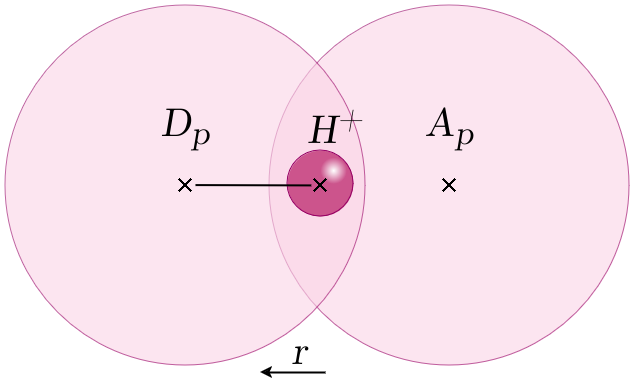
\includegraphics[width=0.4\textwidth]{./img/DrawModel1.png}
\caption{Descripción del modelo de transferencia de protones $H^+$.}
\label{fig:drawmodel}
\end{figure}

En donde $D_p$ y $A_p$ hacen referencia a las partículas donador y aceptor respectivamente, la coordenada $r$ es la distancia del protón al centro de los enlaces. \cite{DynamicalTheoryPTS}. \\
En las descripciones teóricas de la transferencia de protones, a menudo el hidrógeno es representado moviéndose a través de un pozo de doble potencial unidimensional \cite{Enzymes, Krishtalik2000}. 
\\

A continuación se presenta un modelo particular de potencial para el sistema de transferencia de protones, en donde la descripción está dada por la coordenada del protón $r \in [-1.5 \,\,\mathring{A}, 1.5 \,\,\mathring{A}]$.
A cada tiempo $t$ el valor del potencial $V(r,t)$\marginpar{Para simplificar la lectura se utiliza $V(r,t)$ para referirse al potencial $V_{GS}$ en la \autoref{eq:hamApprox}.} está dado por el estado base, que es el eigenvalor más bajo de la siguiente matriz:

\begin{equation}
  \label{eq:matrixPot}
  \begin{pmatrix}
    U_1(r,R(t)) &   V \\
    V           & U_2(r,R(t))+X(t)
  \end{pmatrix}.
\end{equation}

En donde $U_1(r,R(t))$ y  $U_2(r,R(t))$ son potenciales de oscilador armónico, y $V$ es una constante de acoplamiento electrónico.

\begin{equation}
  \label{eq:U1}
  U_1(r,R(t))=\frac{1}{2}m\omega_1^2\left( r + \frac{R(t)}{2} \right)^2,
\end{equation}

\begin{equation}
  \label{eq:U2}
  U_2(r,R(t))=\frac{1}{2}m\omega_2^2\left( r - \frac{R(t)}{2} \right)^2.
\end{equation}

En las ecuaciones de potenciales de oscilador armónico, $m$ se refiere a la masa del protón, $\omega_1$ y $\omega_2$  son las frecuencias del potencial armónico del protón. Los términos $U_1(r,R(t))$ y  $U_2(r,R(t))$ están desplazados mediante un término de energía dependiente del tiempo $X(t)$, y un termino de distancia dependiente del tiempo $R(t)$. La dinámica de $X(t)$ corresponde a las fluctuaciones del entorno, mientras que $R(t)$ representa las vibraciones de los sitios donantes y aceptores de protones \cite{Main:2021}:

\begin{equation}
  \label{eq:X(t)}
  X(t)=\lambda \cos(\omega_xt+\theta_x)+X_{eq},
\end{equation}

\begin{equation}
  \label{eq:R(t)}
  R(t)=(R_0-R_{eq})\cos(\omega_Rt + \theta_R) + R_{eq}.
\end{equation}
En donde $\lambda$ es la amplitud del sesgo de energía, $X_{eq}$ es el sesgo energético de equilibrio, $\omega_x$ es la frecuencia de las oscilaciones de polarización de energía, $\theta_x$ es una fase inicial aleatoria; $R_{eq}$ es la distancia de equilibrio entre los mínimos de los potenciales armónicos, $R_0$ es el desplazamiento inicial desde el equilibrio, $\omega_R$ es la frecuencia de las oscilaciones de la distancia donante-aceptor de protones y $\theta_R$ es una fase inicial aleatoria \cite{Main:2021}.



\begin{figure}[ht]
  \centering
  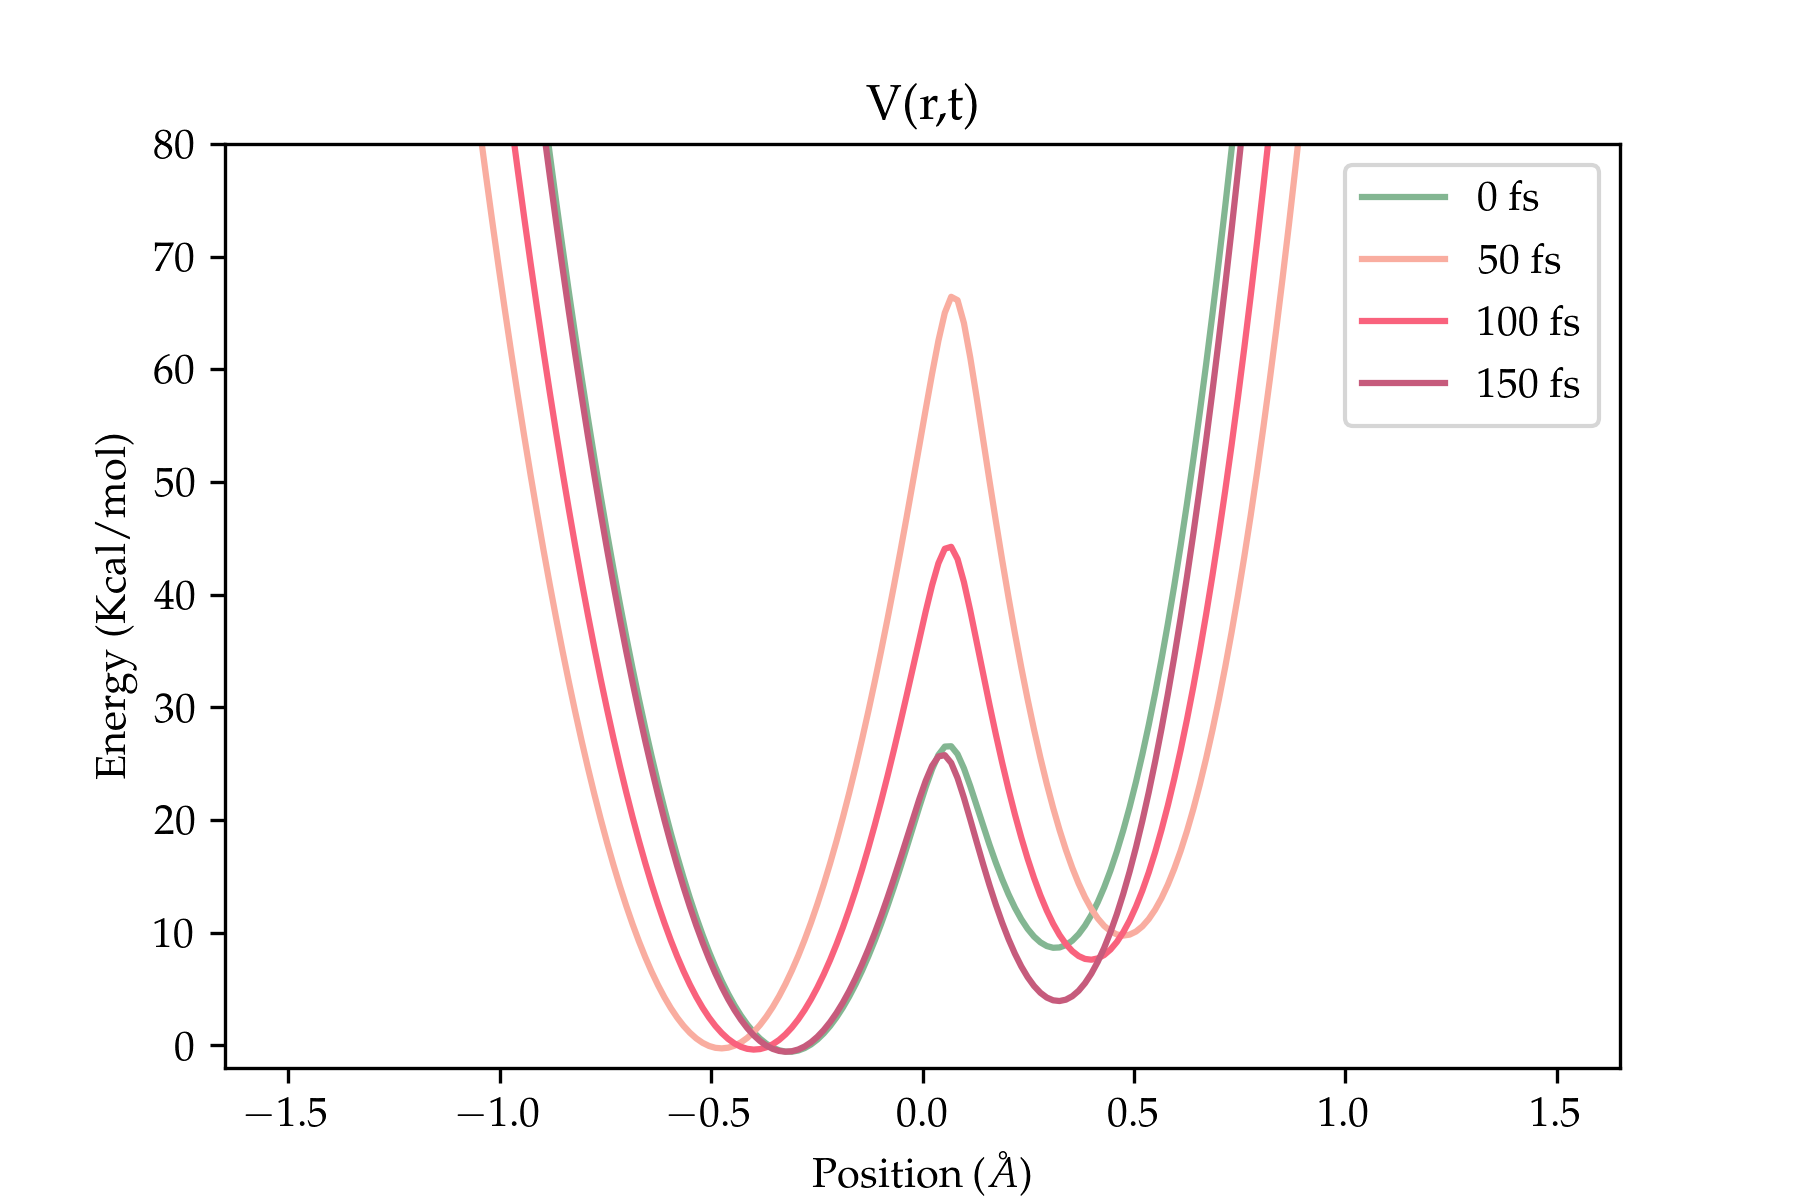
\includegraphics[width=1\textwidth]{./img/ExamplesPotential1.png}
  \caption{Potencial $V(r,t)$ a diferentes tiempos.}
  \label{fig:drawPot}
\end{figure}

La \autoref{fig:drawPot} muestra un ejemplo de potencial $V(r,t)$ generado con la implementación de las ecuaciones anteriores. Los parámetros de potencial utilizados se muestran en la \autoref{tab:ValuesPlot1}.
\\
La \autoref{fig:drawGSandES} muestra el estado base que se toma como el potencial, es decir, el primer estado excitado del sistema correspondiente al eigenvalor más bajo de la matriz en la \autoref{eq:matrixPot}, y los potenciales de oscilador armónico \autoref{eq:U1} y \autoref{eq:U2} a un tiempo $t$.

\begin{figure}[ht]
  \centering
  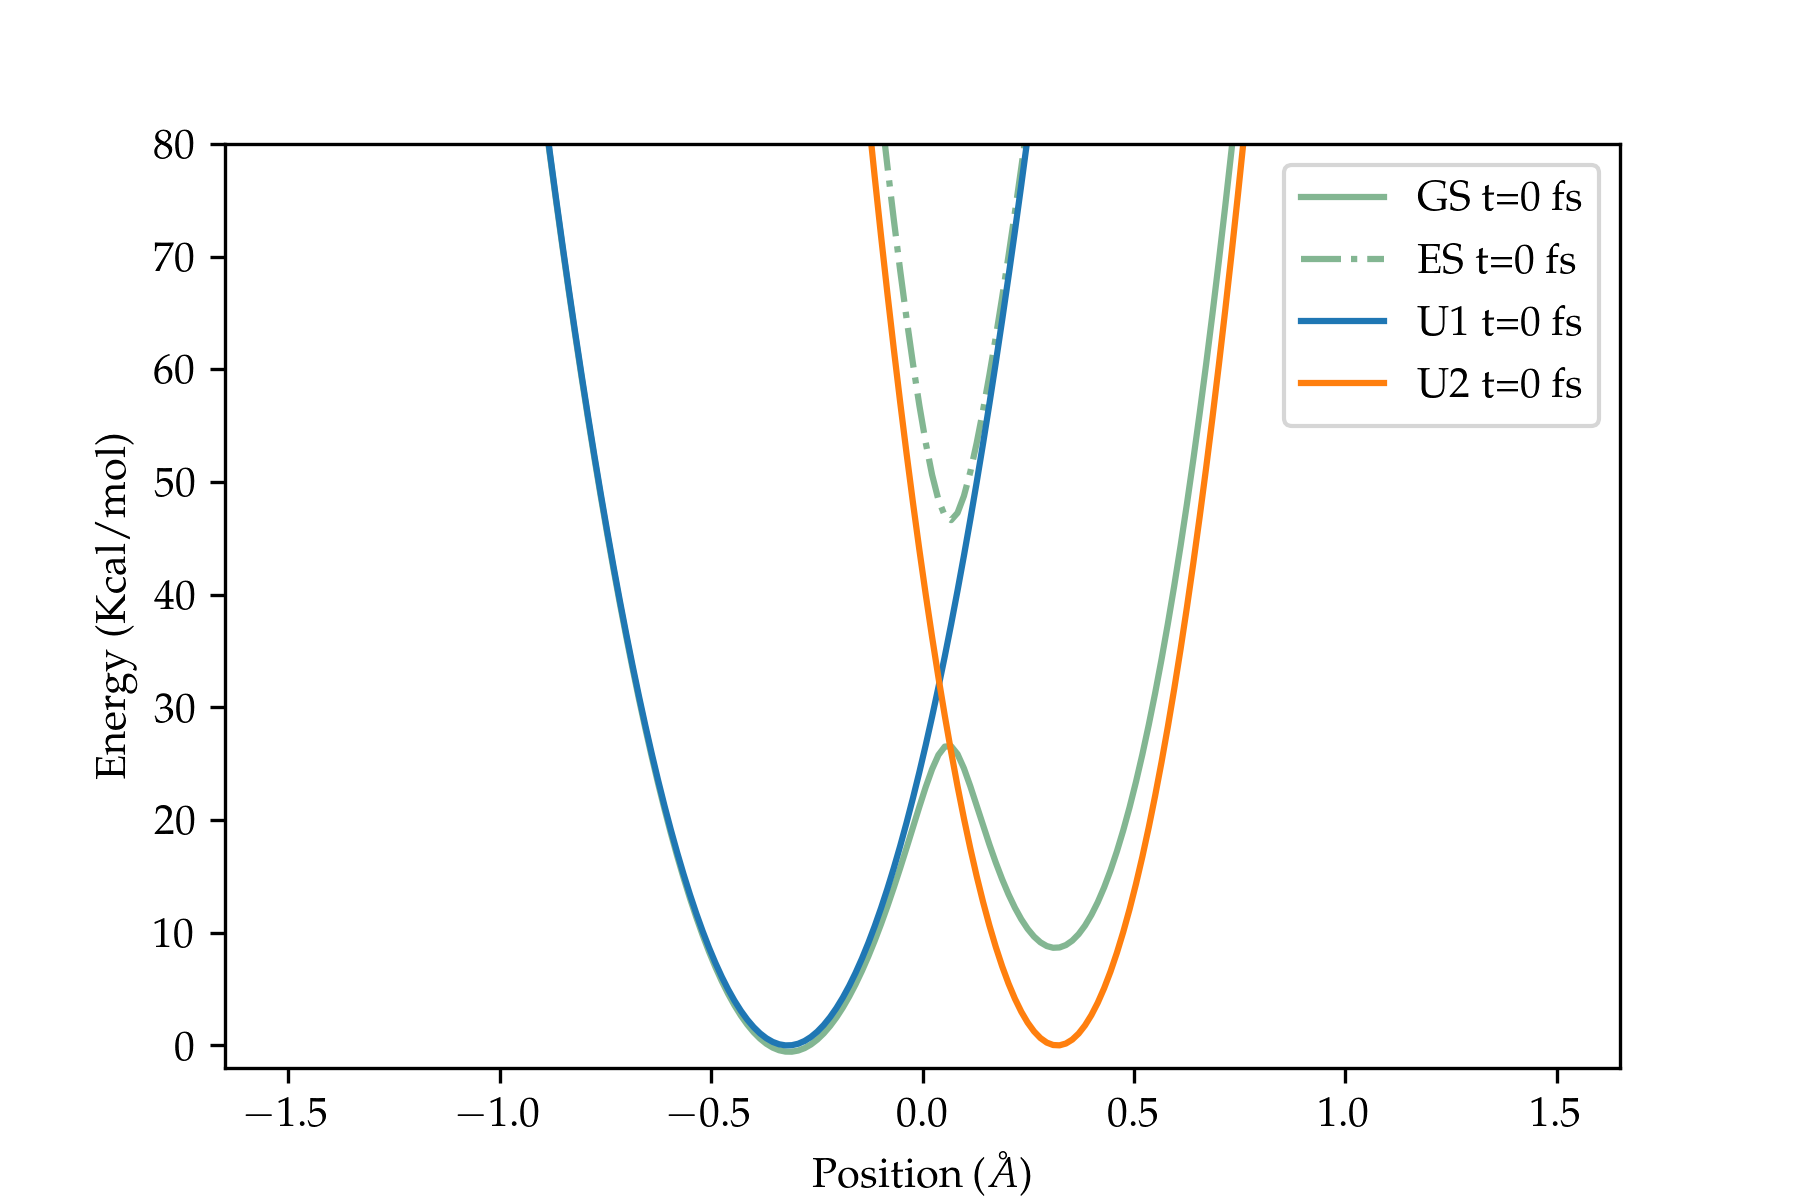
\includegraphics[width=1\textwidth]{./img/ExamplesGSandES.png}
  \caption{Estado base (GS), primer estado excitado (ES) y potenciales armónicos $U_1(r,R(t))$ y $U_2(r, R(t))$ al tiempo $t=0$.}
  \label{fig:drawGSandES}
\end{figure}


\subsection{Elección de una base ortonormal}

Para proceder con la solución a la \acs{TDSE} \autoref{eq:TDSE ket}, elegimos la base de Fourier como base espectral de funciones ortogonales \cite{Colbert1992}:

\begin{equation}
  \label{eq:eigenfunc}
  \phi_n(r)=\sqrt{\frac{2}{b-a}}\sin \frac{n\pi(r-a)}{b-a} \,\,\,\,\, n=1,\dots,N,
\end{equation}

que es ortonormal $\langle \phi_j|\phi_k\rangle = \delta_{jk}$ y completa si $n \to \infty$. 
Con los parámetros $a=-1.5\,\,\mathring{A}$, $b=1.5\,\,\mathring{A}$ y $N=200$ para la implementación numérica, es decir, que el espacio reducido de Hilbert del sistema tiene una dimensión de $N=200$.
La \autoref{fig:Phi_n} muestra las primeras cinco funciones ortogonales de la base, las funciones $\phi_n$ están construidas para que se cumpla: $\phi_n(r=r_0=a)=\phi_n(r=r_{N+1}=b)=0$.

\begin{figure}[ht]
  \centering
  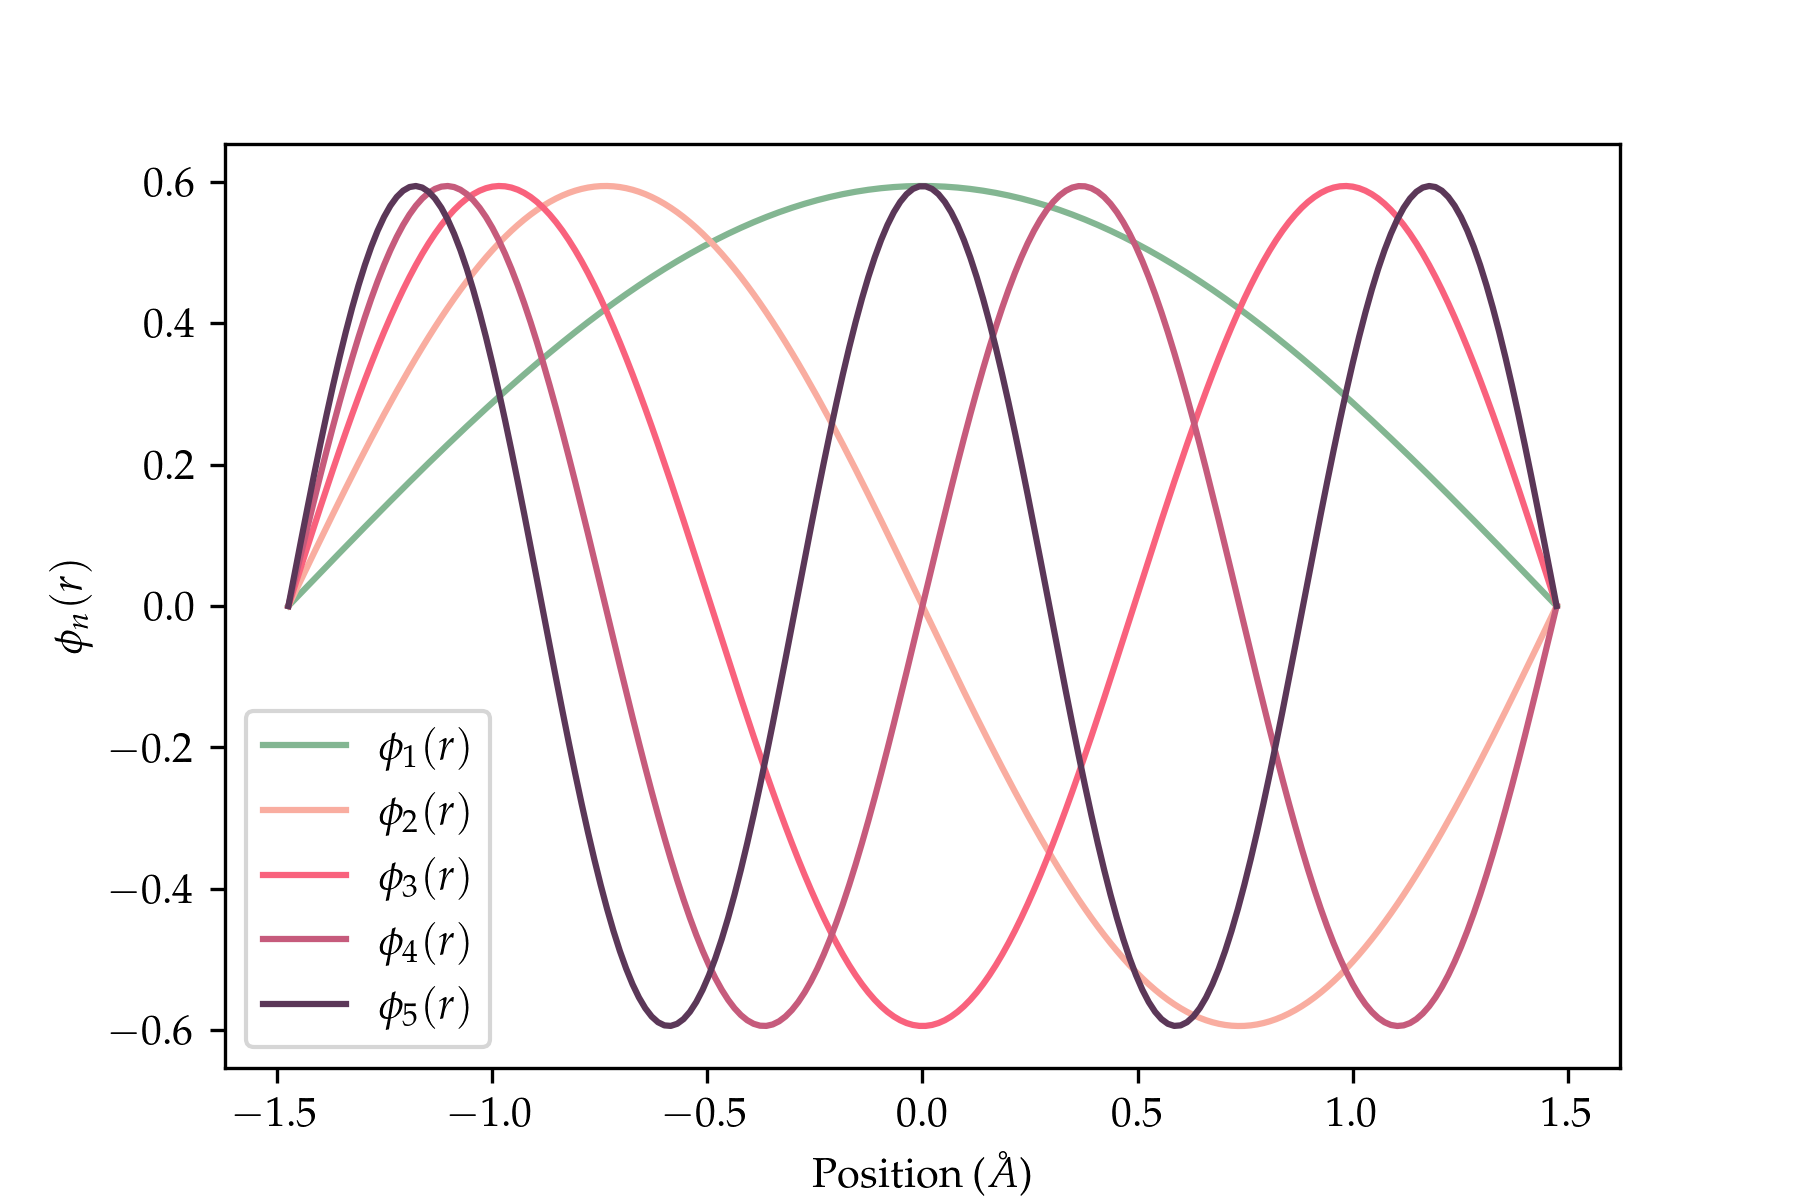
\includegraphics[width=1\textwidth]{./img/Phi_n1.png}
  \caption{Funciones ortogonales $\phi_n(r)$ para $n=1,\dots,5$.}
  \label{fig:Phi_n}
\end{figure}

Dada esta base, los siguientes elementos de matriz pueden ser calculados de manera exacta:

\begin{equation}
  \label{eq:trash}
  \bra{\phi_j}\ket{\phi_k} = \delta_{jk},
\end{equation}

\begin{equation}
  \label{eq:trash1}
  \bra{\phi_j}\frac{d}{d r}\ket{\phi_k} = mod(j-k,2)\frac{4}{b-a}\left(\frac{jk}{j^2 - k^2}\right)\,\,\,\text{con } j\neq k,
\end{equation}

\begin{equation}
  \label{eq:trash2}
  \bra{\phi_j}\frac{d^2}{d r^2}\ket{\phi_k} = -\left( \frac{j\pi}{b-a} \right)^2 \delta_{jk}.
\end{equation}

La energía cinética está dada por $T= -\frac{\hbar^2}{2m}\frac{d^2}{d r^2}$, usando la \autoref{eq:trash2} se tiene que los elementos de matriz de energía cinética en la base espectral están dados por:
\begin{equation}
  \label{eq:T_phi0}
  T^{\phi}_{jk} = \bra{\phi_j}T\ket{\phi_k} = -\frac{\hbar^2}{2m}\bra{\phi_j}\frac{d^2}{d r^2}\ket{\phi_k},
\end{equation}
\begin{equation}
  \label{eq:T_phi}
  T^{\phi}_{jk} = \frac{\hbar^2}{2m} \left( \frac{j\pi}{b-a} \right)^2 \delta_{jk}.
\end{equation}

\subsection{Representación del operador espacial $\hat{r}$ en la base espectral}

La matriz que representa al operador espacial $\hat{r}$ en la base de funciones ortogonales $\{\phi_n \}_{n=1}^{N}$ está dada por $\bra{\phi_j}r\ket{\phi_k}$, sin embargo, para hacer más sencilla la diagonalización en el siguiente paso, se usará la siguiente transformación \cite{Hans}:

\begin{equation}
  \label{eq:trash3}
  f(r) = \cos{\pi\frac{(r-r_0)}{b-a}},
\end{equation}

\noindent de esta manera, los elementos de matriz están dados por:

\begin{equation}
  \label{eq:trash4}
  F_{jk} = \bra{\phi_j}f(r)\ket{\phi_k} = \frac{1}{2}(\delta_{j,k+1}+ \delta_{j,k-1}) = \frac{1}{2}
  \begin{pmatrix}
0 & 1 & 0 & \ldots\\
1 & 0 & 1 & \ldots \\
0 & 1 & 0 & \ldots \\
\vdots & \vdots & \vdots & \ddots
\end{pmatrix}.
\end{equation}

\subsection{Diagonalización mediante una transformación unitaria para definir la malla}

La matriz de la \autoref{eq:trash4} es una matriz simétrica con entradas reales, por el teorema espectral de dimensión finita, puede ser diagonalizada por una matriz ortogonal:

\begin{equation}
  \label{eq:trash5}
  \Phi_{j\alpha} = \sqrt{\frac{2}{N+1}}\sin{\frac{j\alpha \pi}{N+1}},
\end{equation}

\noindent que además es hermitiana y unitaria:
\begin{align}
  \label{eq:unitaryproof}
  \{\Phi^{\dagger} \Phi\}_{jk} &= \{\Phi \Phi\}_{jk}, \\
                      &= \frac{2}{N+1} \sum_{\alpha}^{N} \sin{\pi\frac{j\alpha}{N+1}}\sin{\pi\frac{k\alpha}{N+1}} =
                        \begin{cases}
                          1 & \text{si}\ j=k \\
                          0 & \text{si}\ j\neq k
                        \end{cases}.
\end{align}


\noindent y sus eigenvalores están dados por \cite{Noschese2012}:

\begin{equation}
  \label{eq:trash7}
  f_{\alpha} = \cos{\frac{\alpha \pi}{N+1}},
\end{equation}

\noindent de esta manera, los puntos en la malla están definidos por:

\begin{align}
  \label{eq:malla}
  r_{\alpha} &= f^{-1}(f_{\alpha}) = r_0 + \frac{b-a}{\pi}\arccos{f_{\alpha}} = r_0 + \alpha \frac{b-a}{N+1}, \nonumber\\
  r_{\alpha} &= r_0 + \alpha \Delta r,
\end{align}

\noindent con $\alpha=1,2,\dots,N$ y $\Delta r = \frac{b-a}{N+1}$.


\subsection{Representación del Hamiltoniano en la base pseudo-espectral}

La \autoref{eq:trash5} permite pasar de la base espectral de las funciones ortogonales a la base pseudo-espectral de las funciones localizadas espacialmente. La base de las funciones pseudo-espectrales se puede escribir explícitamente usando la \autoref{eq:11.43}:\footnote{El desarrollo de la \autoref{eq:11.43} es una corrección al resultado presentado en las notas \cite{Hans} de Hans-Dieter Meyer.}

\begin{align}
  \theta_{\alpha}(r) & = \sum_{j=1}^{N}\phi_j(x)\Phi_{j\alpha}, \label{eq:trash9}\\
    & = \sum_{j=1}^{N} \sqrt{\frac{2}{b-a}}\sin{\frac{j\pi(r-r_0)}{b-a}}\sqrt{\frac{2}{N+1}} \sin{\frac{j\alpha \pi}{N+1}}, \label{eq:trash10}\\
                     & = \frac{2}{\sqrt{(b-a)(N+1)}}\sum_{j=1}^{N}\sin{\frac{j\pi(r-r_0)}{b-a}}\sin{\frac{j\alpha \pi}{N+1}}, \label{eq:trash11} \\
  & \text{\noindent usando identidades trigonométricas de multiplicación a suma:} \nonumber \\
    & = \frac{2}{\sqrt{(b-a)(N+1)}}\sum_{j=1}^{N} \frac{1}{2}\left\{
\cos{j\pi \left(\frac{r-r_0}{b-a} - \frac{\alpha}{N+1}\right)} 
-
\cos{j\pi \left(\frac{r-r_0}{b-a} + \frac{\alpha}{N+1}\right)}
\right\}, \label{eq:trash11} \\
& = \frac{1}{\sqrt{(b-a)(n+1)}} \left\{
\sum_{j=1}^{N}
\cos{j\pi \left(\frac{r-r_0}{b-a} - \frac{\alpha}{N+1}\right)} 
-
\sum_{j=1}^{N}
\cos{j\pi \left(\frac{r-r_0}{b-a} + \frac{\alpha}{N+1}\right)}
                                 \right\}, \label{eq:trash12} \\
   & \text{\noindent de acuerdo a \autoref{A:proof}:} \nonumber \\
\theta_{\alpha}(r) & = \frac{1}{\sqrt{(b-a)(n+1)}} \left\{
\cos{\frac{N+1}{2} \pi \left(\frac{r-r_0}{b-a} - \frac{\alpha}{N+1}\right) }
\frac{\sin{\frac{N}{2}}\pi \left(\frac{r-r_0}{b-a} - \frac{\alpha}{N+1}\right)}{\sin\frac{1}{2}\pi \left(\frac{r-r_0}{b-a} - \frac{\alpha}{N+1}\right)} \right. \nonumber \\
&-
\left. \cos{\frac{N+1}{2} \pi \left(\frac{r-r_0}{b-a} + \frac{\alpha}{N+1}\right) }
\frac{\sin{\frac{N}{2}}\pi \left(\frac{r-r_0}{b-a} + \frac{\alpha}{N+1}\right)}{\sin\frac{1}{2}\pi \left(\frac{r-r_0}{b-a} + \frac{\alpha}{N+1}\right)}\right\}. \label{eq:trash13}
\end{align}

La \autoref{fig:theta_n} muestra algunas funciones base pseudo-espectrales. Estas funciones tienen un valor distinto de cero únicamente en el punto $r_{i=\alpha}$, como se esperaba por las propiedades descritas en la sección \autoref{sec:ps-basis}.

\begin{figure}[ht]
  \centering
  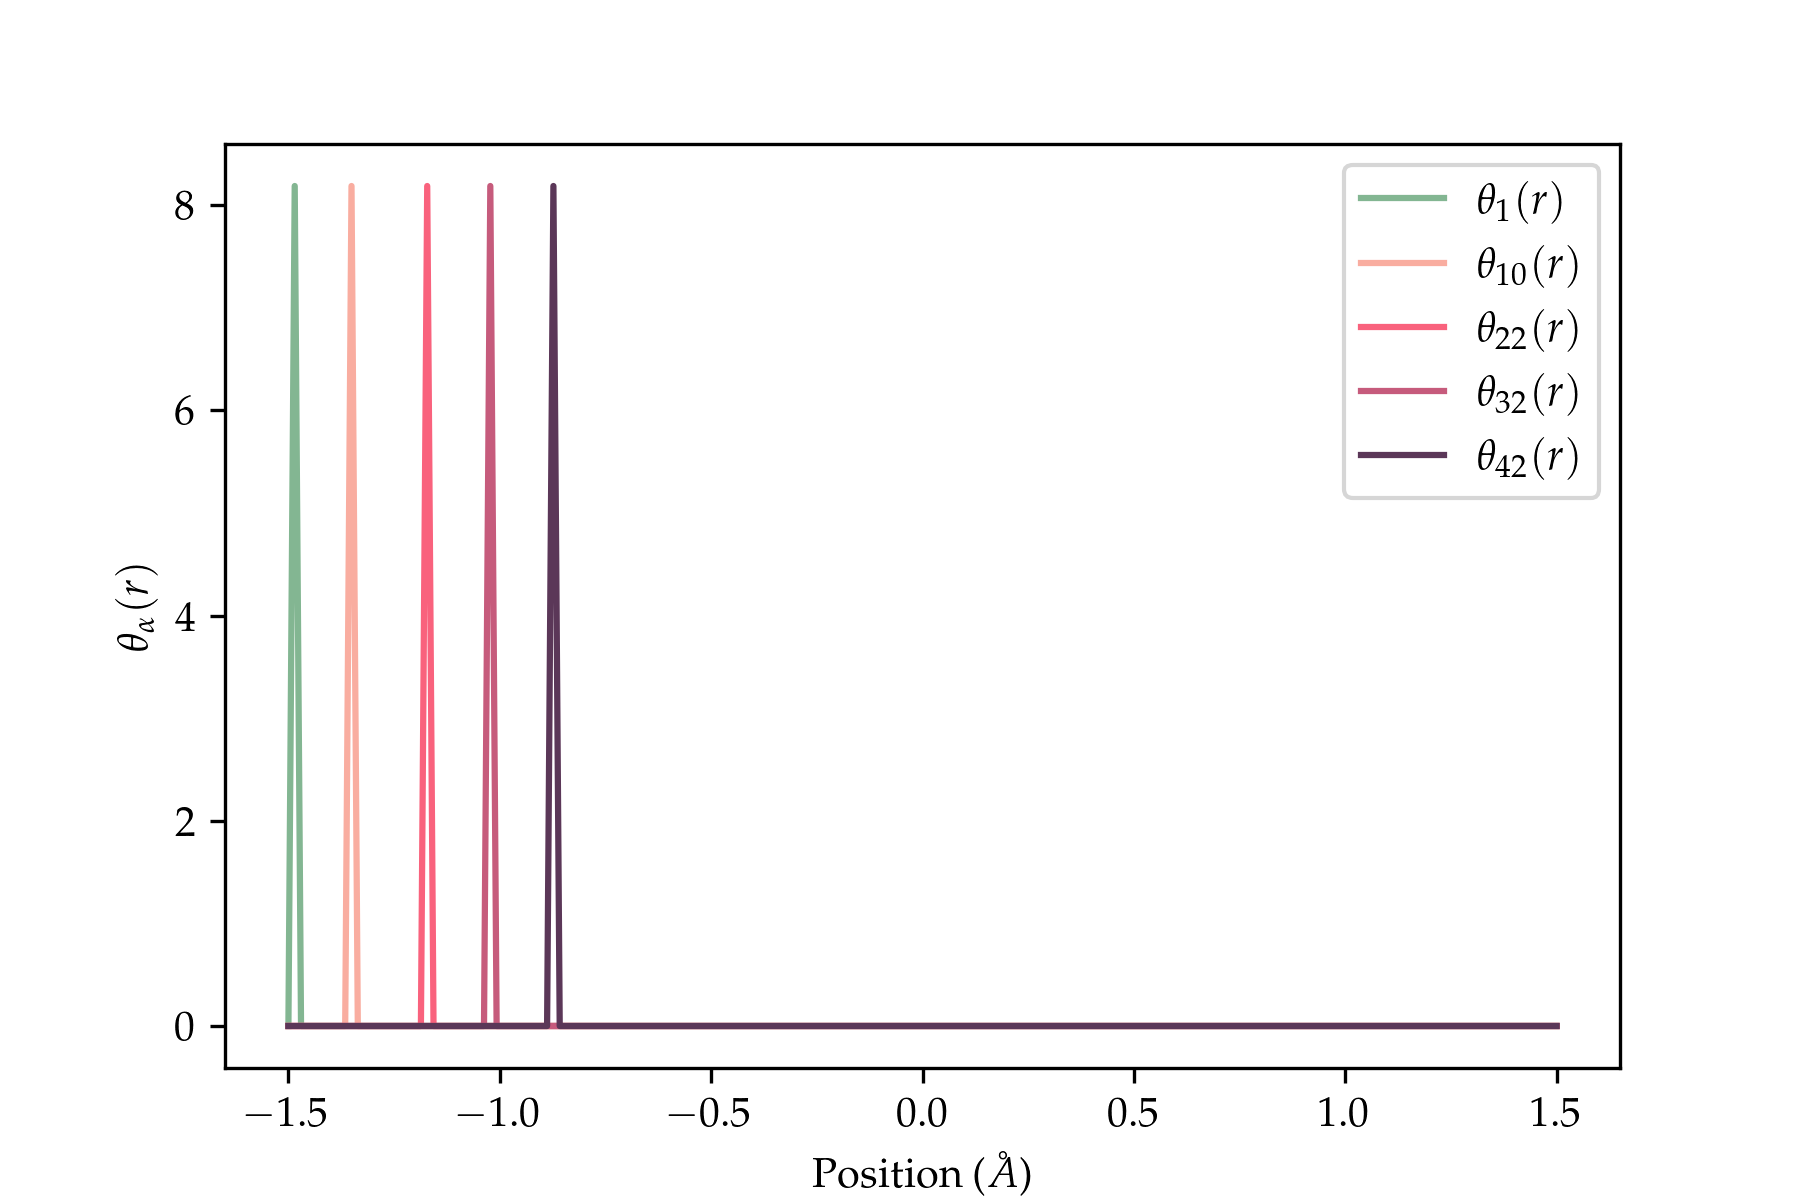
\includegraphics[width=1\textwidth]{./img/theta_n1.png}
  \caption{Funciones ortogonales $\theta_{\alpha}(r)$ en la malla $\{r_i\}_{i=1}^{N}$ para $\alpha=1,10,22,32,42$.}
  \label{fig:theta_n}
\end{figure}

La representación de la matriz de energía potencial en la base pseudo-espectral es simple, pues 
las funciones $\{\theta_{\alpha}\}$ son localizadas en el espacio de posiciones y cumplen la condición de ortogonalidad $\bra{\theta_{\alpha}}\ket{\theta_{\beta}}= \delta_{\alpha \beta}$, así:

\begin{equation}
  \label{eq:V_DVR}
  V^{\theta}_{ij}= \bra{\theta_i}V(\hat{r})\ket{\theta_j}=V(r_i)\delta_{ij},
\end{equation}

\noindent $V^{\theta}\in \mathcal{M}_{200\times200}(\mathbb{R})$ es una matriz diagonal.
\\
Dado un tiempo $t$, los elementos de la diagonal $V^{\theta}_{ii}$ están dados por $V(r_i,t)$ (\autoref{eq:matrixPot}), con $i=0,..,199$.
\\
\\
Escribir directamente la matriz de energía cinética en la base pseudo-espectral es, en general, complicado, por ello comúnmente se calcula en la base espectral y se utiliza la matriz de transformación unitaria \autoref{eq:trash5} para escribirla en la base pseudo-espectral:

\begin{equation}
  \label{eq:trash6}
  T^{\theta} = \Phi T^{\phi} \Phi,
\end{equation}

\noindent en donde $T^{\phi}$ está dada por la \autoref{eq:T_phi}, de esta manera, la matriz del Hamiltoniano en la base pseudo-espectral al tiempo $t$ es:

\begin{equation}
  \label{eq:H_DVR}
  H(t)^{\theta} = V(t)^{\theta}+T^{\theta},
\end{equation}
en donde el Hamiltoniano tiene dependencia temporal debido a que el potencial del sistema es dependiente del tiempo.

\subsection{Propagación de un paquete de onda}

Sea un paquete de onda Gaussiana definido por:

\begin{equation}
  \label{eq:psi_00}
g(r)=\frac{1}{\sigma\sqrt{2\pi}}\exp{\frac{-1}{2}\frac{(r-\mu)^2}{\sigma^2}},
\end{equation}

\noindent con valores $\mu$ y $\sigma$ valores aleatorios elegidos entre $(-0.5,-0.5)\,\, \mathring{A}$ y $(0.1,0.3)\,\, \mathring{A}$ respectivamente. \\

La \autoref{eq:psi_00} puede escribirse como suma de las funciones pseudo-espectrales \autoref{eq:trash13} en la malla definida por los puntos en la \autoref{eq:malla} multiplicados por coeficientes complejos $C_i$. De esta manera, se puede definir una onda inicial al tiempo $t=0$ como:

\begin{equation}
  \label{eq:psi_0}
\psi(r,0)=\sum_{i=1}^{N}C_i \cdot \theta_{i}(r),
\end{equation}
con $C_i$ elegidos de tal forma que $\bra{\psi(r,0)}\ket{\psi(r,0)}=1$.
\begin{figure}[!htbp]
  \centering
  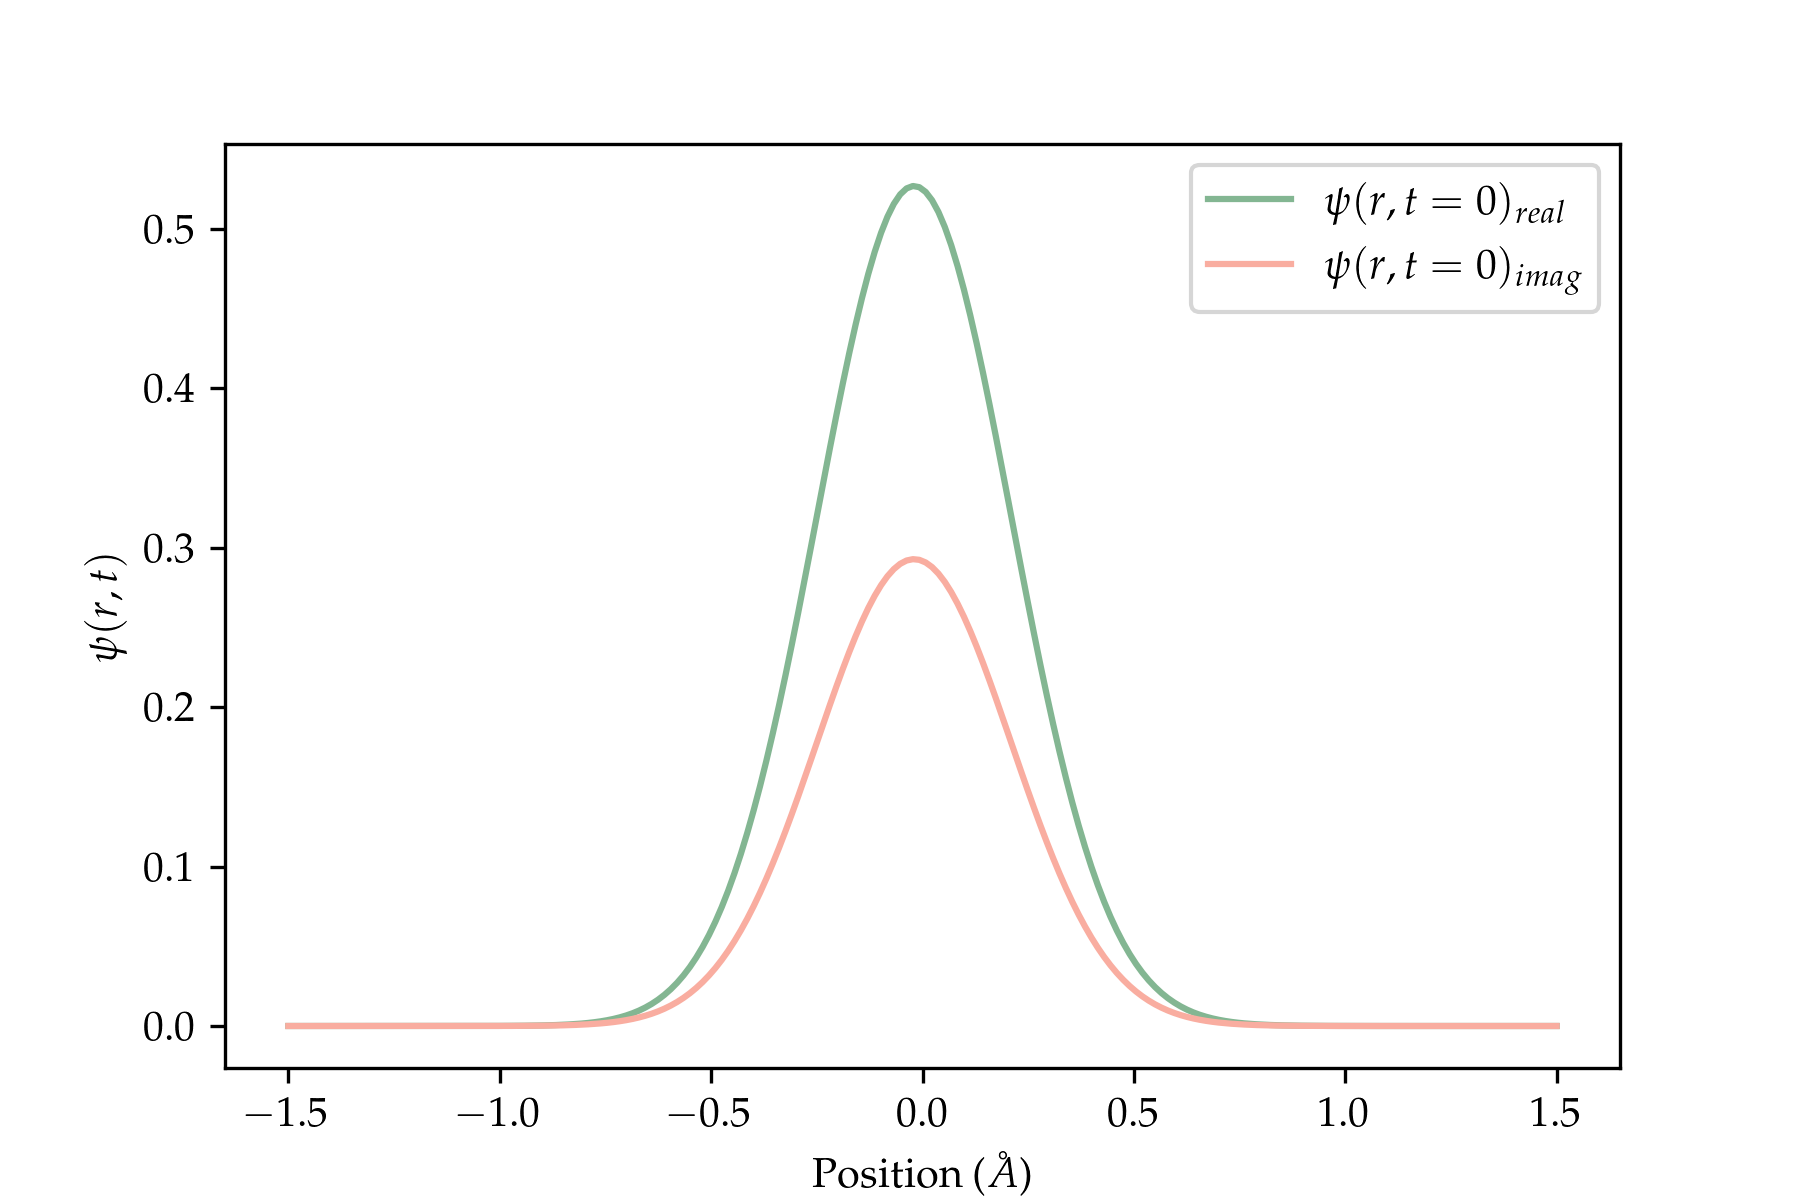
\includegraphics[width=0.9\textwidth]{./img/psi_01}
  \caption{Paquete inicial de onda al tiempo $t=0$. Parte real y compleja.}
  \label{fig:psi_0}
\end{figure}

Si se toma un intervalo de tiempo $\Delta t$ lo suficientemente pequeño, como para que el potencial se pueda considerar constante en ese intervalo de tiempo ($\approx 1\,\,fs$ para el sistema en cuestión considerando el periodo de las frecuencias $\omega_1$ y $\omega_2$), la evolución temporal del paquete de onda está dado por la \autoref{eq:U IT}:
\begin{equation}
  \label{eq:wp_ev}
  \psi(r,t)=\exp{-iH^{\theta}t/\hbar}\psi(r,t-1),
\end{equation}

Si $H^{\theta} = UDU^{-1}$, con $D$ una matriz diagonal:
$$ \psi(r,t) = \exp{-iUDU^{-1}t/\hbar}\psi(r,t-1)$$  ,
así,
\begin{equation}
  \label{eq:psi_t}
\psi(r,t) = U\exp{\frac{-it}{\hbar}D}U^{-1}\psi(r,t-1).
\end{equation}

En donde la matriz $U$ está formada por los $N$ eigenvectores de $H^{\theta}$ como vectores columna, y:
$$D=U^{-1}H^{\theta}U.$$
\\

La \autoref{fig:psi_evre} y la \autoref{fig:psi_evim} muestran algunas ondas de la evolución de la parte real e imaginaria del paquete de onda en intervalos de $50\,fs$ a lo largo de $150\,fs$, obtenidas con la \autoref{eq:psi_t}. En la \autoref{fig:dens_ev} se muestra la evolución temporal de la densidad del protón.\\
Las siguientes animaciones muestran la evolución temporal con el potencial incluido. \\
\href{https://github.com/Jessi-MM/LSTM_PropagatorLearning/blob/main/src/Animation/gifs/animation-dens%26pot.gif}{\faPlayCircle[regular] Evolución temporal: potencial y densidad de la función de onda} \\
\href{https://github.com/Jessi-MM/LSTM_PropagatorLearning/blob/main/src/Animation/gifs/animation-all.gif}{\faPlayCircle[regular] Evolución temporal: potencial, parte real y compleja de la función de onda y su densidad}

\begin{figure}[!htbp]
  \centering
  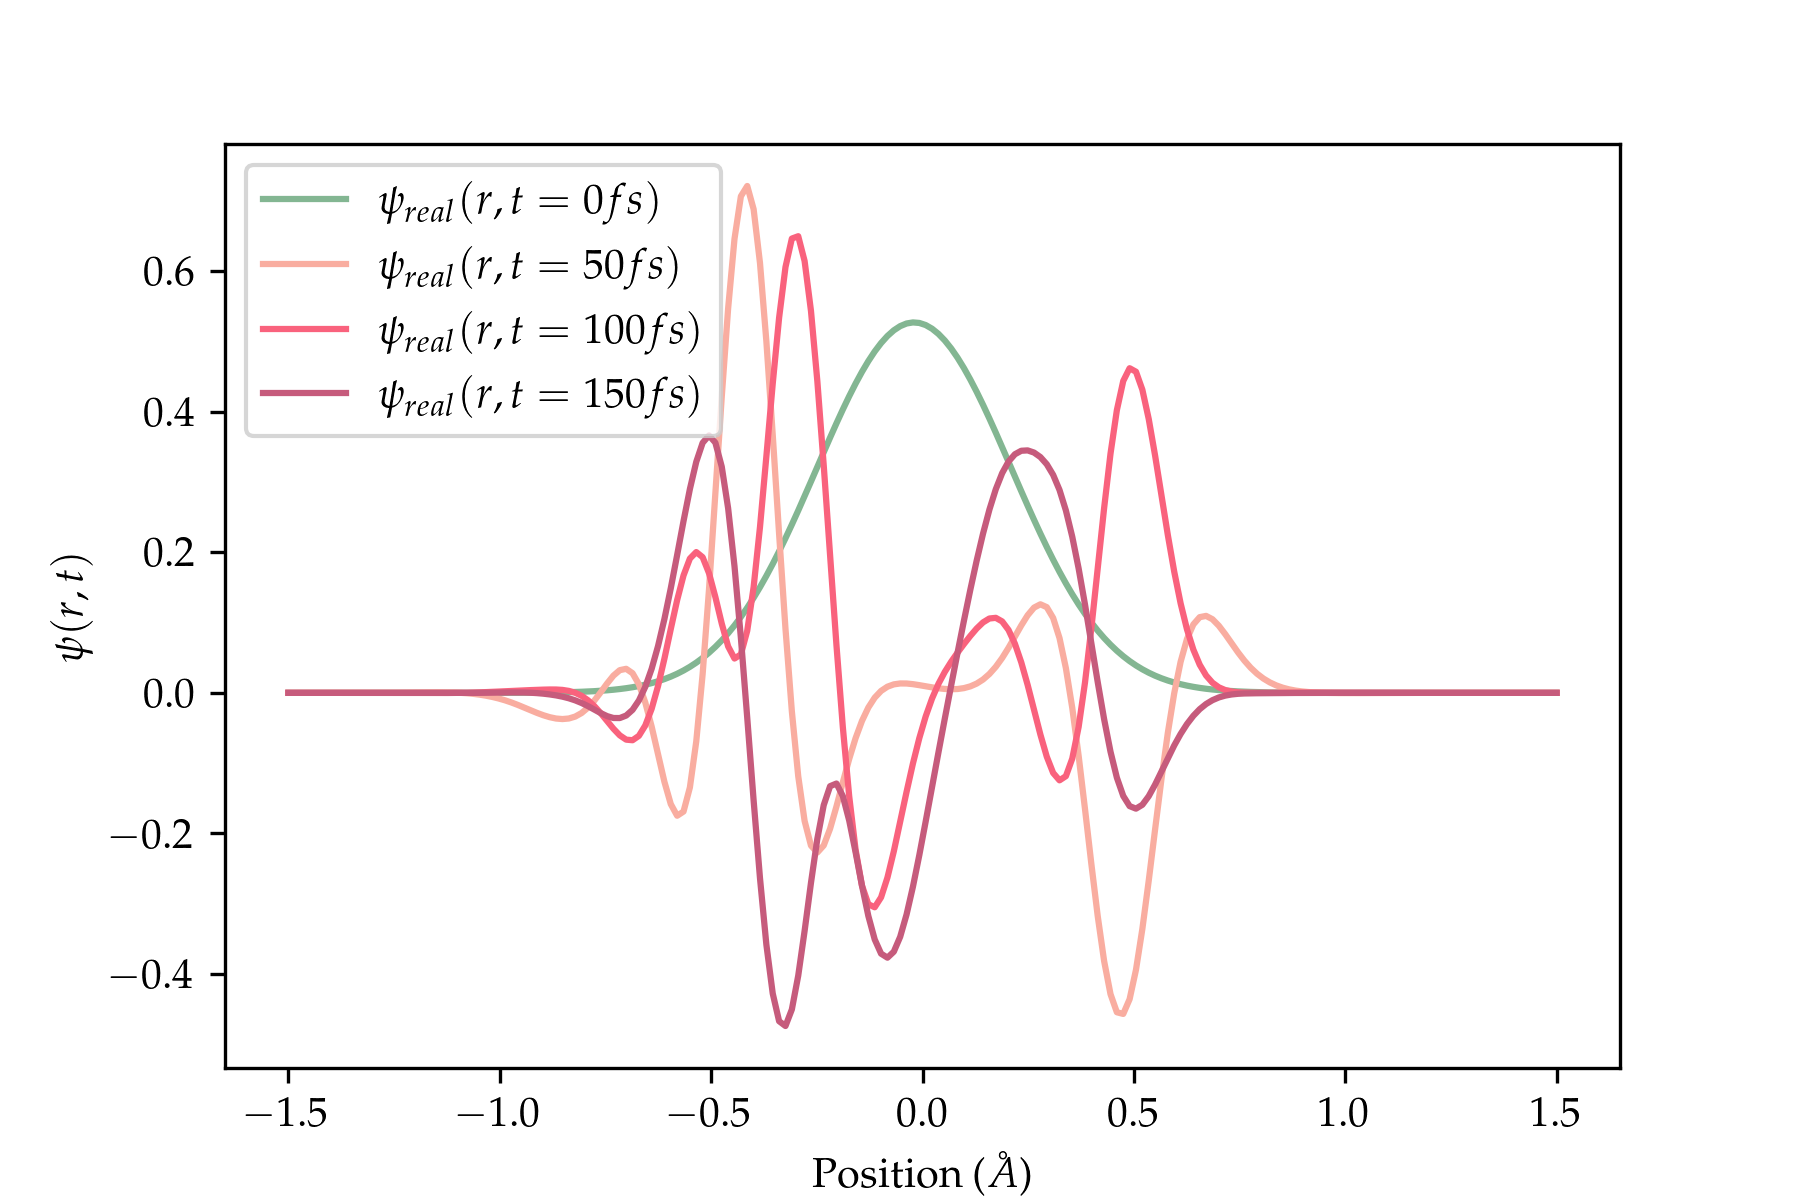
\includegraphics[width=1\textwidth]{./img/psi_ev1imag}
  \caption{Propagación del paquete de onda $\psi(r,t)$ parte real.}
  \label{fig:psi_evre}
\end{figure}

\begin{figure}[!htbp]
  \centering
  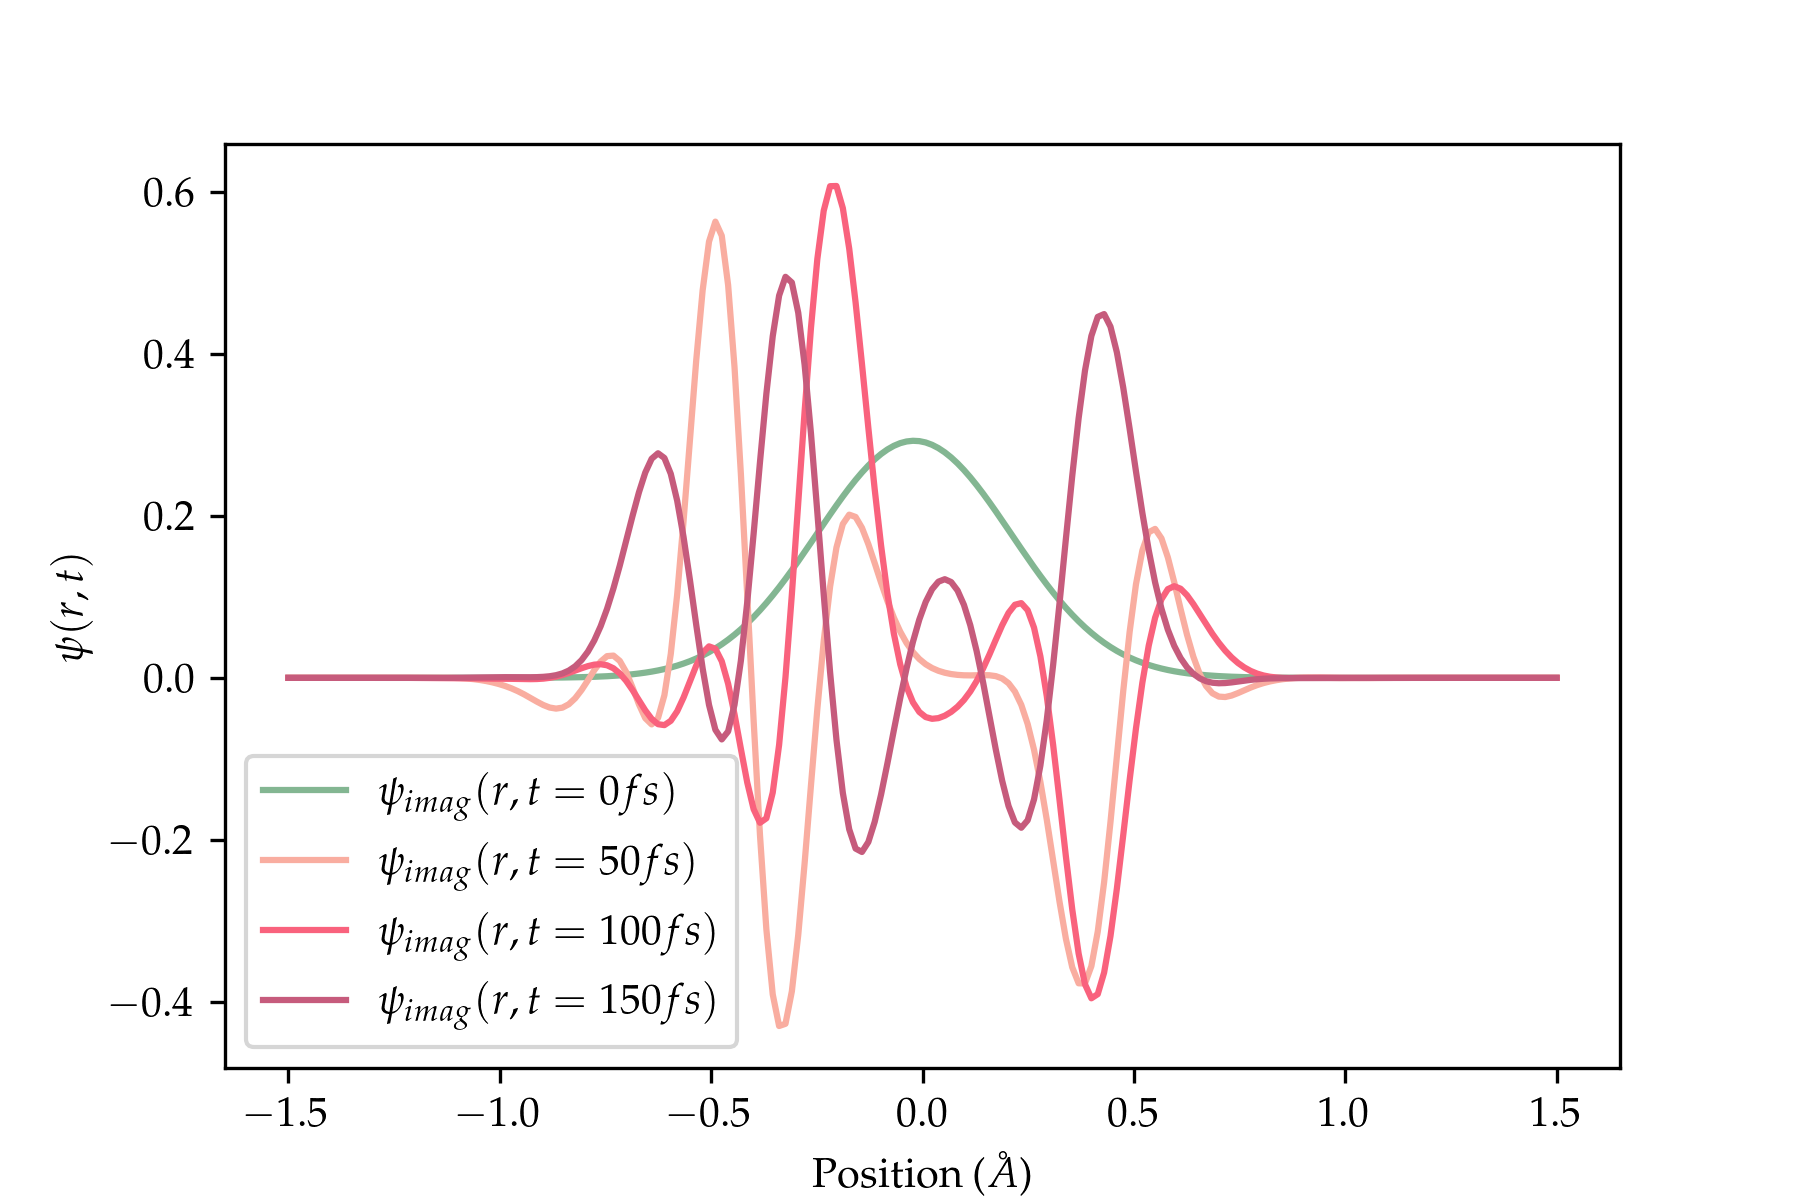
\includegraphics[width=1\textwidth]{./img/psi_ev1real}
  \caption{Propagación del paquete de onda $\psi(r,t)$ parte imaginaria.}
  \label{fig:psi_evim}
\end{figure}

\begin{figure}[!htbp]
  \centering
  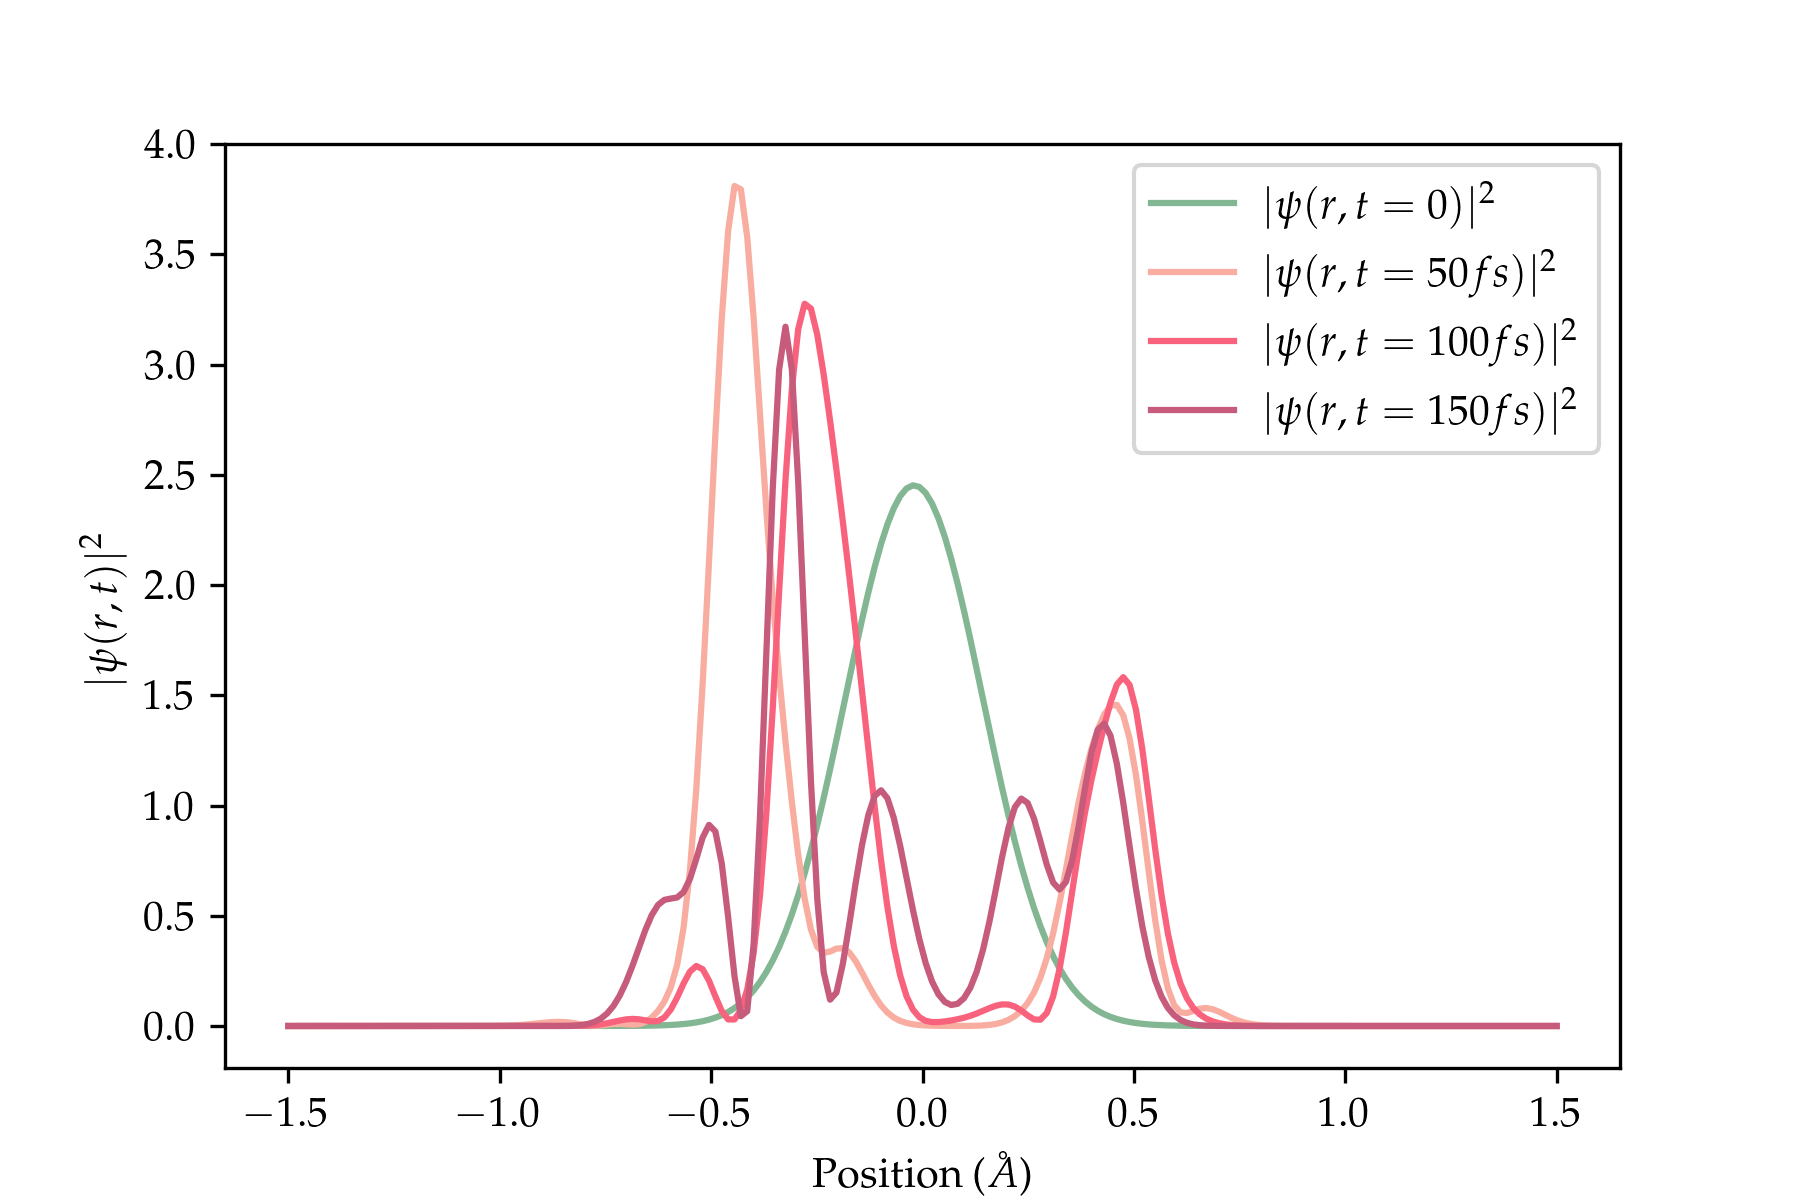
\includegraphics[width=1\textwidth]{./img/dens_ev1}
  \caption{Evolución temporal de la densidad $|\psi(r,t)|^2$.}
  \label{fig:dens_ev}
\end{figure}
